\section{Raspberry Pi 3B+}
This course uses the Raspberry Pi 3B+. The pinout for this device is shown below. Note that some pins have special uses. This pins may not be able to be used as GPIO. Note that the header has a notch to indicate pin 1. It's also important to note the difference board numbering and BCM numbering. Board numbering is the pin count on the headers, i.e. the number shown in the circle in the image. BCM stands for Broadcom SOC channel - and refers to the GPIO number in the descriptions next to number in the circle. For example, board number 3 is GPIO 2, and board number 33 is GPIO number 13. Some pins have special functions. You'll learn about these functions as the course progresses. 

You can only use one board numbering system (BOARD or GPIO) per project, and you usually need to configure this using a method made available in the library.

\begin{figure}[H]
\centering
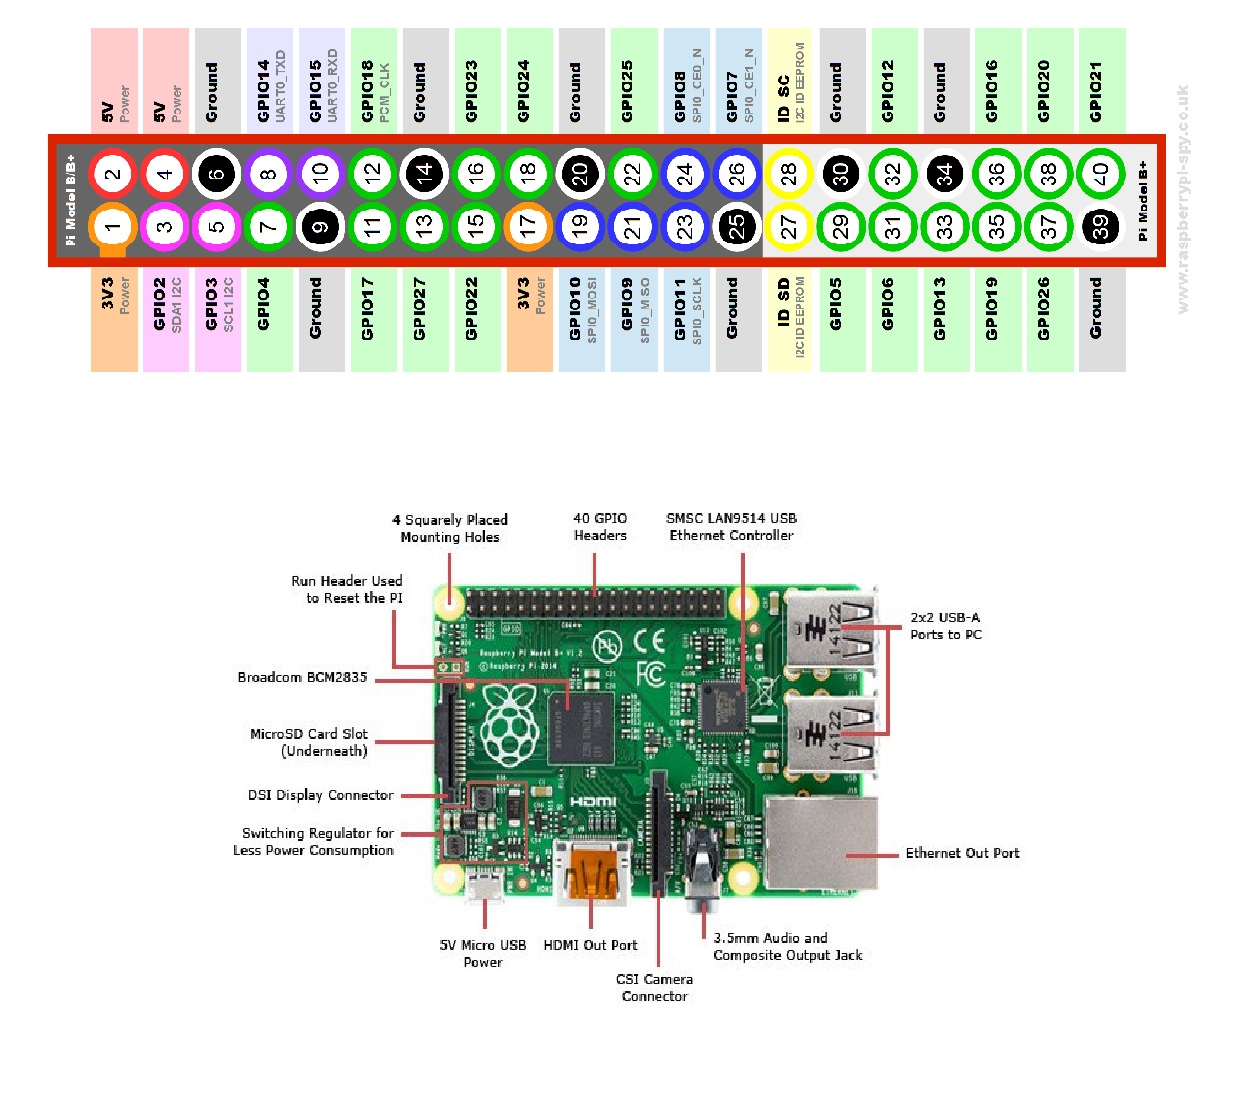
\includegraphics[width=\columnwidth]{Figures/pinout}
\caption{GPIO Header of the B+ \href{https://www.jameco.com/Jameco/workshop/circuitnotes/raspberry-pi-circuit-note.html}{(source)}}
\label{fig:pinout}
\end{figure}

\subsection{Board Modes}
\label{sec:BoardModes}
The Raspberry Pi has a number of "board modes" depending on which library you use for development. Some of these modes include:
\begin{itemize}
    \item BCM Mode\\
    This is the pin numbering that is tied to the Broadcom chip that powers the Raspberry Pi.
    \item GPIO/Physical Mode\\
    This is the pin numbering that matches the physical pin numbering of the header.
    \item WiringPi numbering\\
    WiringPi is a library for writing C/C++ applications on the Raspberry Pi. It has it's own unique pin numbering. It includes a useful function for viewing all the pinouts, numbering, and what their current state is. A screenshot of this function is shown in Figure \ref{fig:gpio-readall}.
\end{itemize}

\begin{figure}[H]
\centering
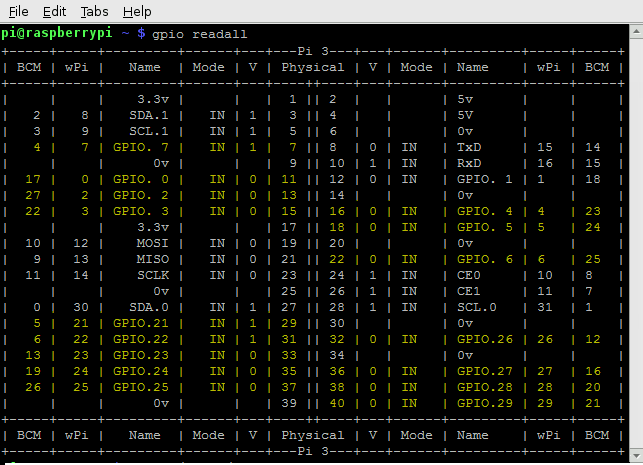
\includegraphics[width=0.6\columnwidth]{Figures/gpio-readall}
\caption{A screenshot of running "gpio readall"}
\label{fig:gpio-readall}
\end{figure}
